

\documentclass{standalone}
\usepackage{tikz}
\usepackage{amsmath}
\usetikzlibrary{positioning, shapes.geometric, arrows}

\usetikzlibrary{shapes.geometric, arrows, positioning, fit}
\tikzstyle{startstop} = [rectangle, rounded corners, minimum width=3cm, minimum height=1cm,text centered, draw=black]
\tikzstyle{io} = [trapezium, trapezium left angle=70, trapezium right angle=110, minimum width=3cm, minimum height=1cm, text centered, draw=black]
\tikzstyle{process} = [rectangle, minimum width=3cm, minimum height=1cm, text centered, text width=3cm, draw=black]
\tikzstyle{decision} = [diamond, minimum width=3cm, minimum height=1cm, text centered, draw=black]
\tikzset{main node/.style={circle,,draw,minimum size=1cm,inner sep=0pt} }
\tikzstyle{arrow} = [thick,->,>=stealth]




\begin{document}

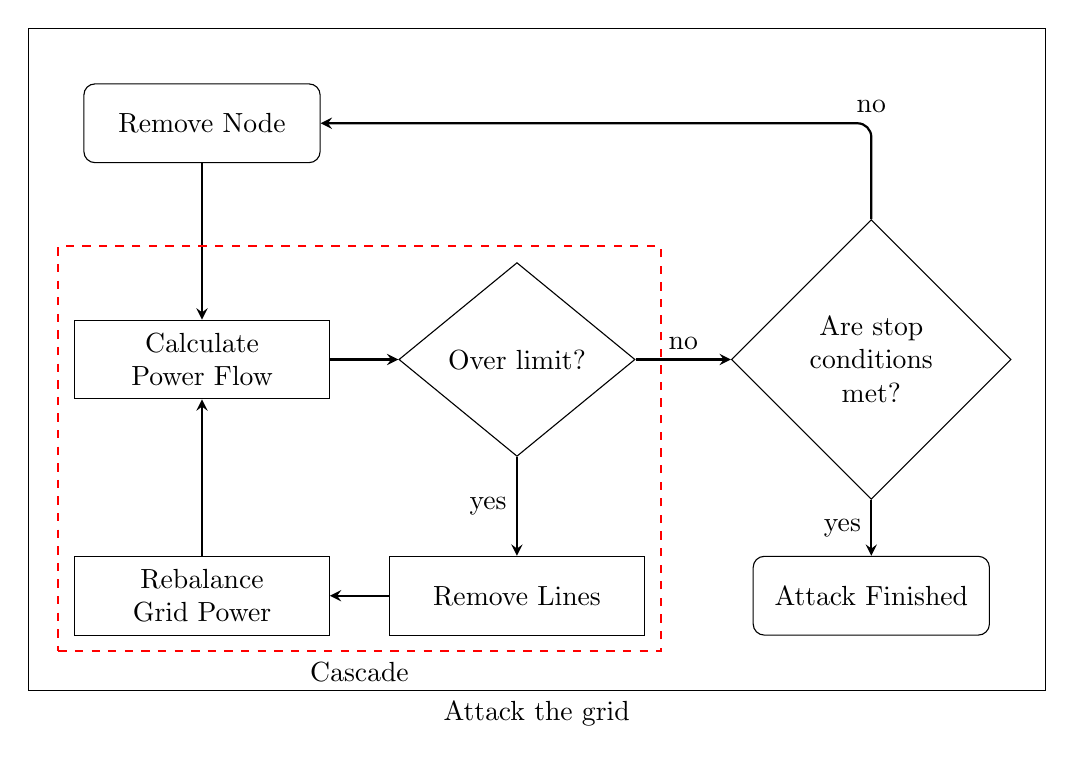
\begin{tikzpicture}[node distance=2cm]

\node (start) [startstop] {Remove Node};
\node (PowCalc) [process, below of=start, yshift = -1cm] {Calculate Power Flow};

\node (OverLim) [decision, right of=PowCalc, xshift = 2cm] {Over limit?};

\node (Remove) [process, below of=OverLim, yshift=-1cm] {Remove Lines};

\node (Rebalance) [process, below of=PowCalc, yshift=-1cm] {Rebalance Grid Power};

\node (stopconds) [decision, right of = OverLim, xshift = 2.5cm, text width=2cm] {Are stop conditions met?};

%\node (CascFin) [decision, right of = OverLim, xshift = 2.5cm, text width=2cm] {CascadeFinsished};
%\node (stopconds) [decision, right of = CascFin, xshift = 2.5cm, text width=2cm] {Are stop conditions met?};



\node (stop) [startstop, below of = stopconds, yshift = -1cm] {Attack Finished};

\draw [arrow] (start) -- (PowCalc);
\draw [arrow] (PowCalc) -- (OverLim);
\draw [arrow] (OverLim) -- node[anchor=east] {yes}(Remove);
\draw [arrow] (Remove) -- (Rebalance);
\draw [arrow] (Rebalance) -- (PowCalc);


\draw [arrow] (OverLim) -- node[anchor=south] {no}(stopconds);

%\draw [arrow] (OverLim) -- node[anchor=south] {no}(CascFin);
%\draw [arrow] (CascFin) -- (stopconds)

 
\draw [arrow,rounded corners=5pt] (stopconds.north) |- node[anchor=south] {no}(start.east);
\draw [arrow] (stopconds) -- node[anchor=east] {yes}(stop);

\node[draw, red,thick,dashed,inner sep=2mm,label=below:Cascade,fit=(PowCalc) (OverLim) (Rebalance) (Remove)] {};

\node[draw, inner sep=7mm,label=below:Attack the grid,fit=(stop) (start)] {};

\end{tikzpicture}


\end{document}

